\documentclass[11pt]{article}
\usepackage[textwidth=18.0cm, textheight=23.0cm, top=2.0cm]{geometry}
\usepackage{pst-all}
\usepackage{amssymb}
\usepackage{tikz}
\usepackage{underscore}\begin{document}
\pagestyle{empty}


ClassName: \underline{\textbf{Class_10.2bp-23}}
\par
BinSize: \underline{\textbf{100 × 100}}
\par
ReduceSize: \underline{\textbf{100 × 100}}
\par
TypeNum: \underline{\textbf{60}}
\par
Num: \underline{\textbf{60}}
\par
OutS: \underline{\textbf{80000}}
\par
InS: \underline{\textbf{69409}}
\par
Rate: \underline{\textbf{0.868}}
\par
UB: \underline{\textbf{8}}
\par
LB0: \underline{\textbf{7}}
\par
LB: \underline{\textbf{8}}
\par
LBWithCut: \underline{\textbf{8}}
\par
NodeCut: \underline{\textbf{0}}
\par
ExtendedNodeCnt: \underline{\textbf{1}}
\par
GenNodeCnt: \underline{\textbf{1}}
\par
PrimalNode: \underline{\textbf{0}}
\par
ColumnCount: \underline{\textbf{61}}
\par
TotalCutCount: \underline{\textbf{0}}
\par
RootCutCount: \underline{\textbf{0}}
\par
LPSolverCnt: \underline{\textbf{53}}
\par
PricingSolverCnt: \underline{\textbf{53}}
\par
BranchAndBoundNum: \underline{\textbf{1}}
\par
isOpt: \underline{\textbf{false}}
\par
TimeOnInitSolution: \underline{\textbf{120.010 s}}
\par
TimeOnPrimal: \underline{\textbf{0.000 s}}
\par
TimeOnPricing: \underline{\textbf{3601.962 s}}
\par
TimeOnRmp: \underline{\textbf{0.094 s}}
\par
TotalTime: \underline{\textbf{3722.128 s}}
\par
\newpage


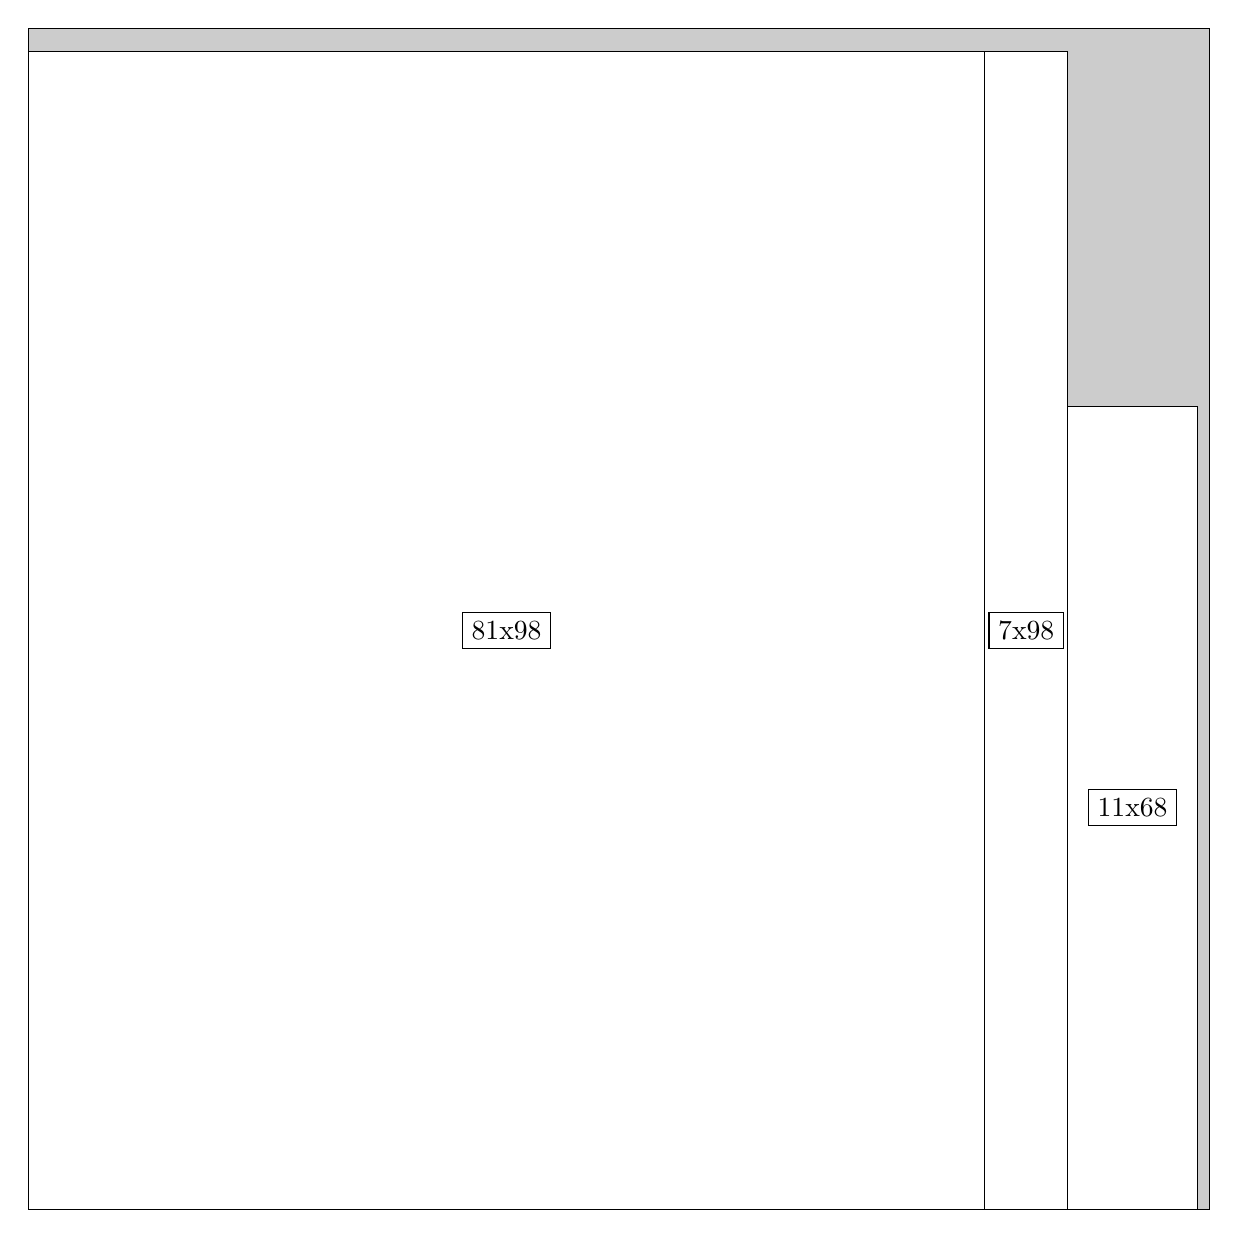
\begin{tikzpicture}[shorten >=1pt,scale=1.0,every node/.style={scale=1.0},->]
\tikzstyle{vertex}=[circle,fill=black!25,minimum size=14pt,inner sep=0pt]
\filldraw[fill=gray!40!white, draw=black] (0,0) rectangle (15.0,15.0);
\foreach \name/\x/\y/\w/\h in {81x98/0.0/0.0/12.15/14.7,11x68/13.2/0.0/1.65/10.2,7x98/12.15/0.0/1.05/14.7}
\filldraw[fill=white!40!white, draw=black] (\x,\y) rectangle node[draw] (\name) {\name} ++(\w,\h);
\end{tikzpicture}


w =81 , h =98 , x =0 , y =0 , v =7938
\par
w =11 , h =68 , x =88 , y =0 , v =748
\par
w =7 , h =98 , x =81 , y =0 , v =686
\par
\newpage


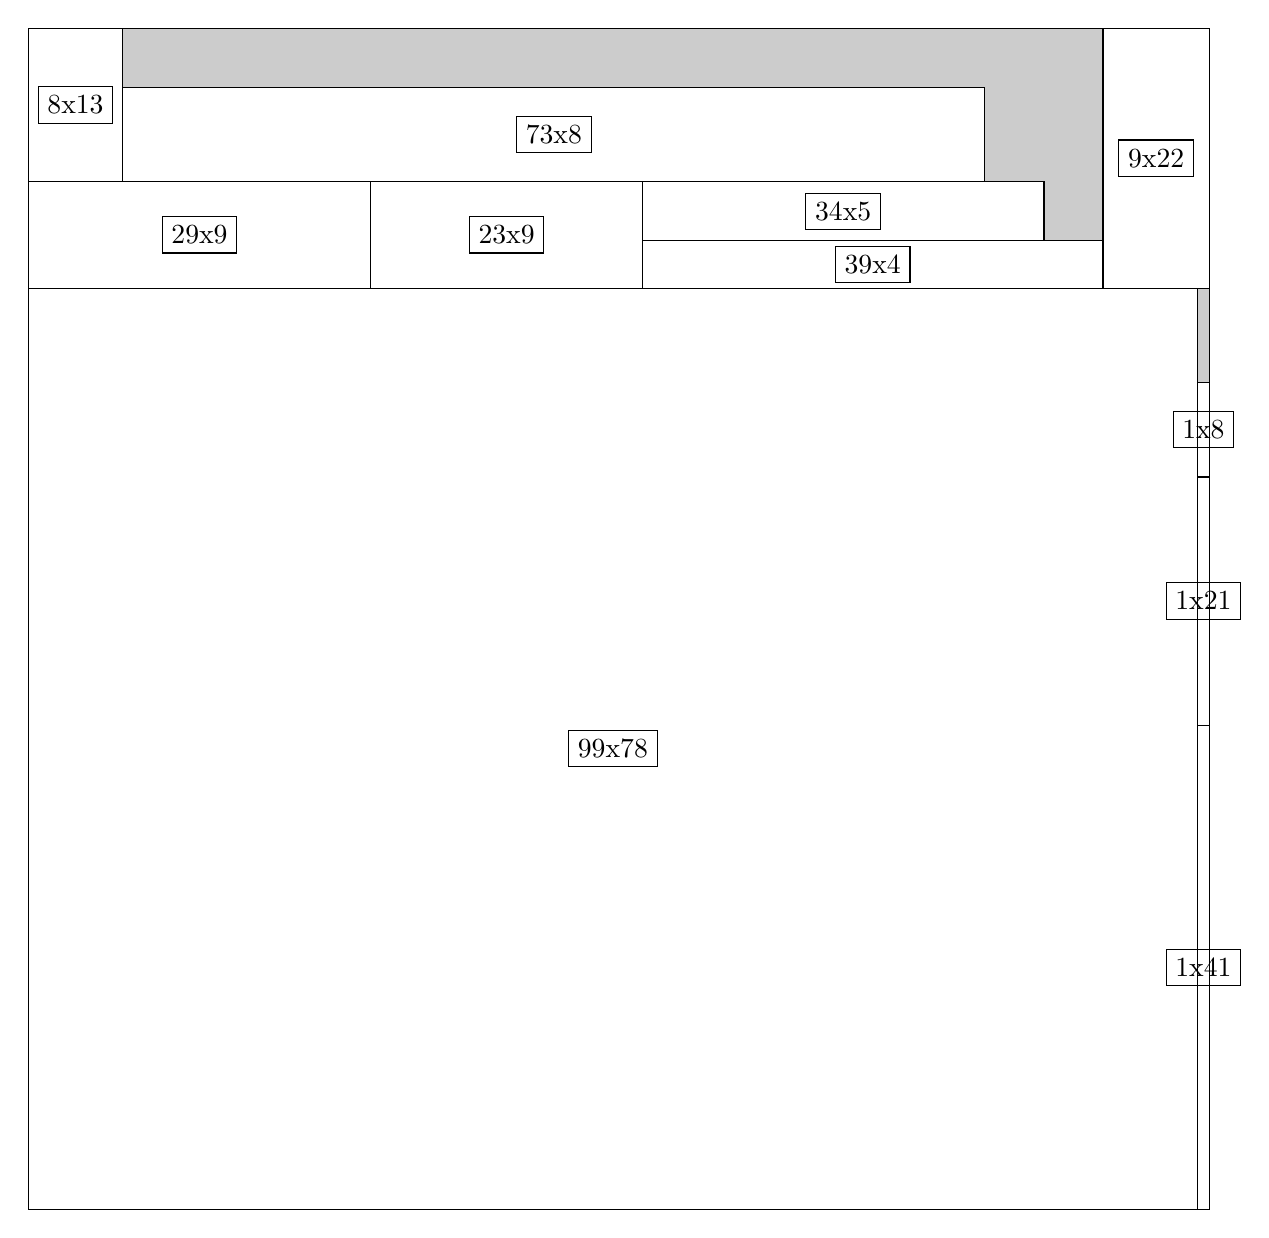
\begin{tikzpicture}[shorten >=1pt,scale=1.0,every node/.style={scale=1.0},->]
\tikzstyle{vertex}=[circle,fill=black!25,minimum size=14pt,inner sep=0pt]
\filldraw[fill=gray!40!white, draw=black] (0,0) rectangle (15.0,15.0);
\foreach \name/\x/\y/\w/\h in {99x78/0.0/0.0/14.85/11.7,29x9/0.0/11.7/4.35/1.3499999999999999,73x8/1.2/13.049999999999999/10.95/1.2,23x9/4.35/11.7/3.4499999999999997/1.3499999999999999,9x22/13.65/11.7/1.3499999999999999/3.3,34x5/7.8/12.299999999999999/5.1/0.75,39x4/7.8/11.7/5.85/0.6,8x13/0.0/13.049999999999999/1.2/1.95,1x41/14.85/0.0/0.15/6.1499999999999995,1x21/14.85/6.1499999999999995/0.15/3.15,1x8/14.85/9.299999999999999/0.15/1.2}
\filldraw[fill=white!40!white, draw=black] (\x,\y) rectangle node[draw] (\name) {\name} ++(\w,\h);
\end{tikzpicture}


w =99 , h =78 , x =0 , y =0 , v =7722
\par
w =29 , h =9 , x =0 , y =78 , v =261
\par
w =73 , h =8 , x =8 , y =87 , v =584
\par
w =23 , h =9 , x =29 , y =78 , v =207
\par
w =9 , h =22 , x =91 , y =78 , v =198
\par
w =34 , h =5 , x =52 , y =82 , v =170
\par
w =39 , h =4 , x =52 , y =78 , v =156
\par
w =8 , h =13 , x =0 , y =87 , v =104
\par
w =1 , h =41 , x =99 , y =0 , v =41
\par
w =1 , h =21 , x =99 , y =41 , v =21
\par
w =1 , h =8 , x =99 , y =62 , v =8
\par
\newpage


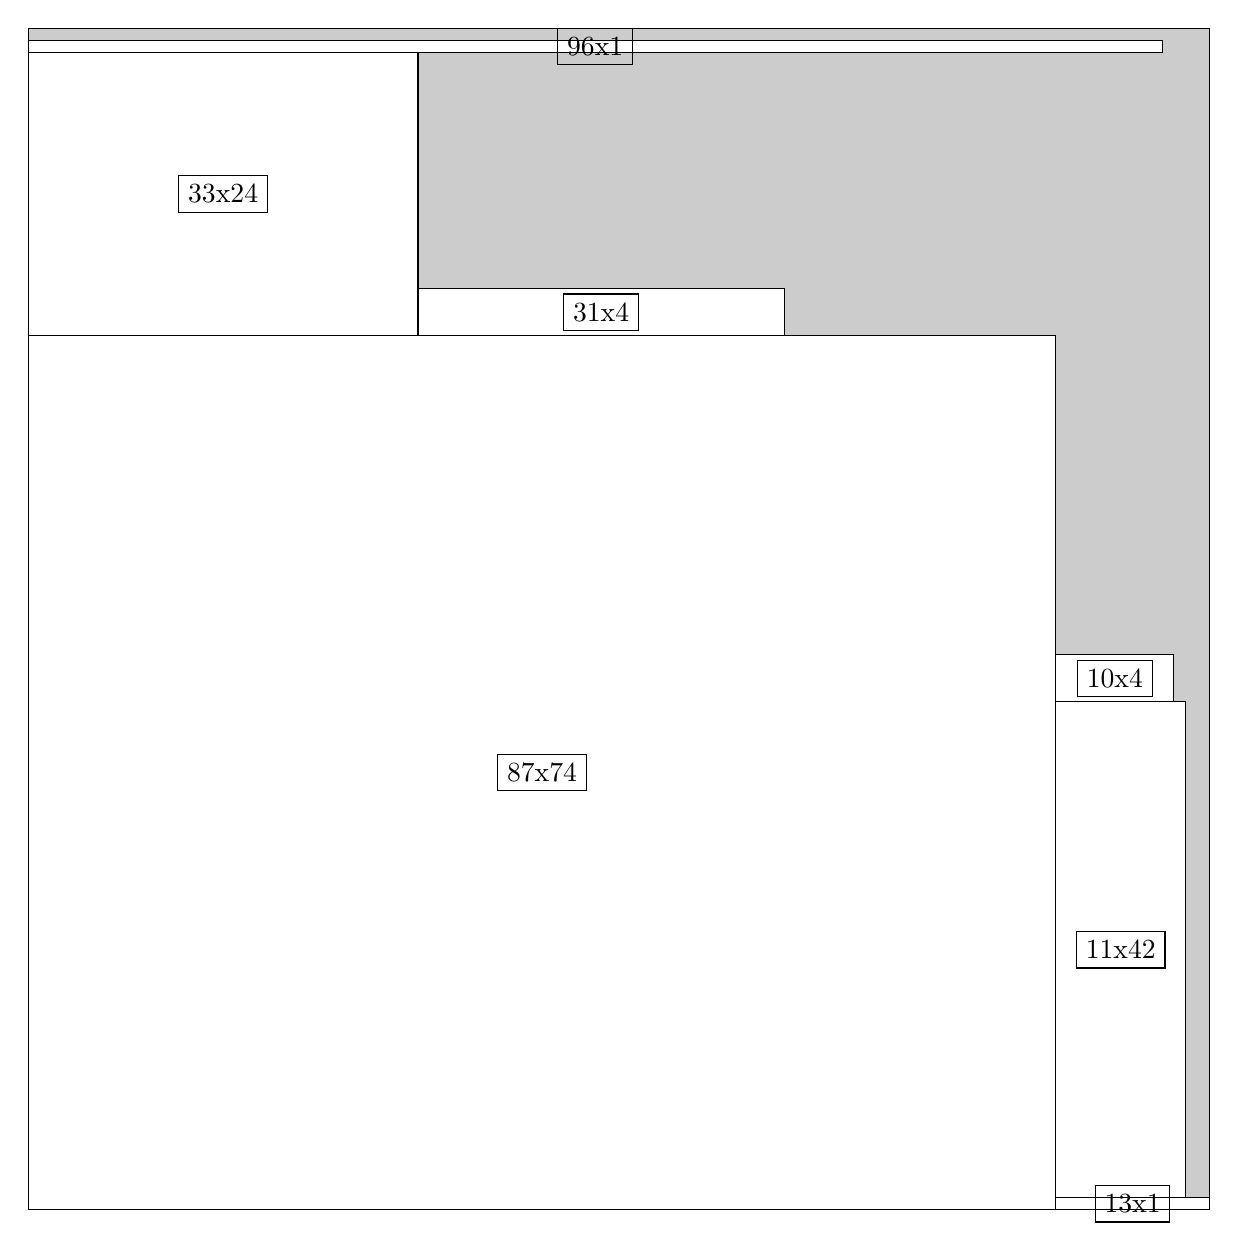
\begin{tikzpicture}[shorten >=1pt,scale=1.0,every node/.style={scale=1.0},->]
\tikzstyle{vertex}=[circle,fill=black!25,minimum size=14pt,inner sep=0pt]
\filldraw[fill=gray!40!white, draw=black] (0,0) rectangle (15.0,15.0);
\foreach \name/\x/\y/\w/\h in {87x74/0.0/0.0/13.049999999999999/11.1,33x24/0.0/11.1/4.95/3.5999999999999996,11x42/13.049999999999999/0.15/1.65/6.3,31x4/4.95/11.1/4.6499999999999995/0.6,96x1/0.0/14.7/14.399999999999999/0.15,10x4/13.049999999999999/6.45/1.5/0.6,13x1/13.049999999999999/0.0/1.95/0.15}
\filldraw[fill=white!40!white, draw=black] (\x,\y) rectangle node[draw] (\name) {\name} ++(\w,\h);
\end{tikzpicture}


w =87 , h =74 , x =0 , y =0 , v =6438
\par
w =33 , h =24 , x =0 , y =74 , v =792
\par
w =11 , h =42 , x =87 , y =1 , v =462
\par
w =31 , h =4 , x =33 , y =74 , v =124
\par
w =96 , h =1 , x =0 , y =98 , v =96
\par
w =10 , h =4 , x =87 , y =43 , v =40
\par
w =13 , h =1 , x =87 , y =0 , v =13
\par
\newpage


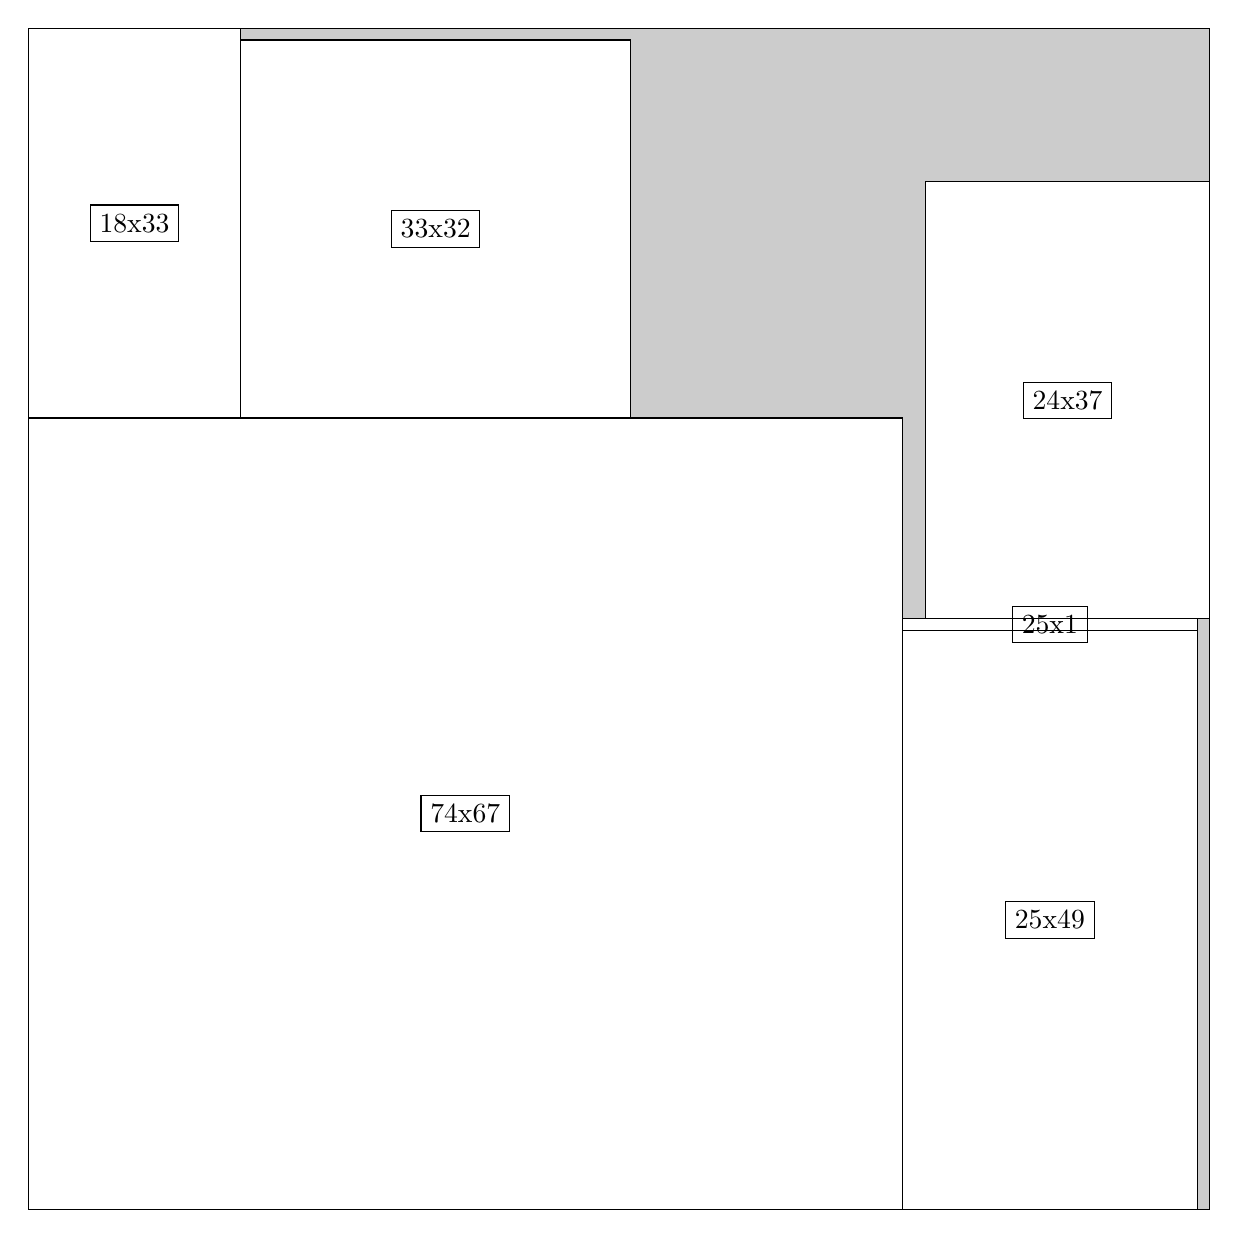
\begin{tikzpicture}[shorten >=1pt,scale=1.0,every node/.style={scale=1.0},->]
\tikzstyle{vertex}=[circle,fill=black!25,minimum size=14pt,inner sep=0pt]
\filldraw[fill=gray!40!white, draw=black] (0,0) rectangle (15.0,15.0);
\foreach \name/\x/\y/\w/\h in {74x67/0.0/0.0/11.1/10.049999999999999,25x49/11.1/0.0/3.75/7.35,33x32/2.6999999999999997/10.049999999999999/4.95/4.8,24x37/11.4/7.5/3.5999999999999996/5.55,18x33/0.0/10.049999999999999/2.6999999999999997/4.95,25x1/11.1/7.35/3.75/0.15}
\filldraw[fill=white!40!white, draw=black] (\x,\y) rectangle node[draw] (\name) {\name} ++(\w,\h);
\end{tikzpicture}


w =74 , h =67 , x =0 , y =0 , v =4958
\par
w =25 , h =49 , x =74 , y =0 , v =1225
\par
w =33 , h =32 , x =18 , y =67 , v =1056
\par
w =24 , h =37 , x =76 , y =50 , v =888
\par
w =18 , h =33 , x =0 , y =67 , v =594
\par
w =25 , h =1 , x =74 , y =49 , v =25
\par
\newpage


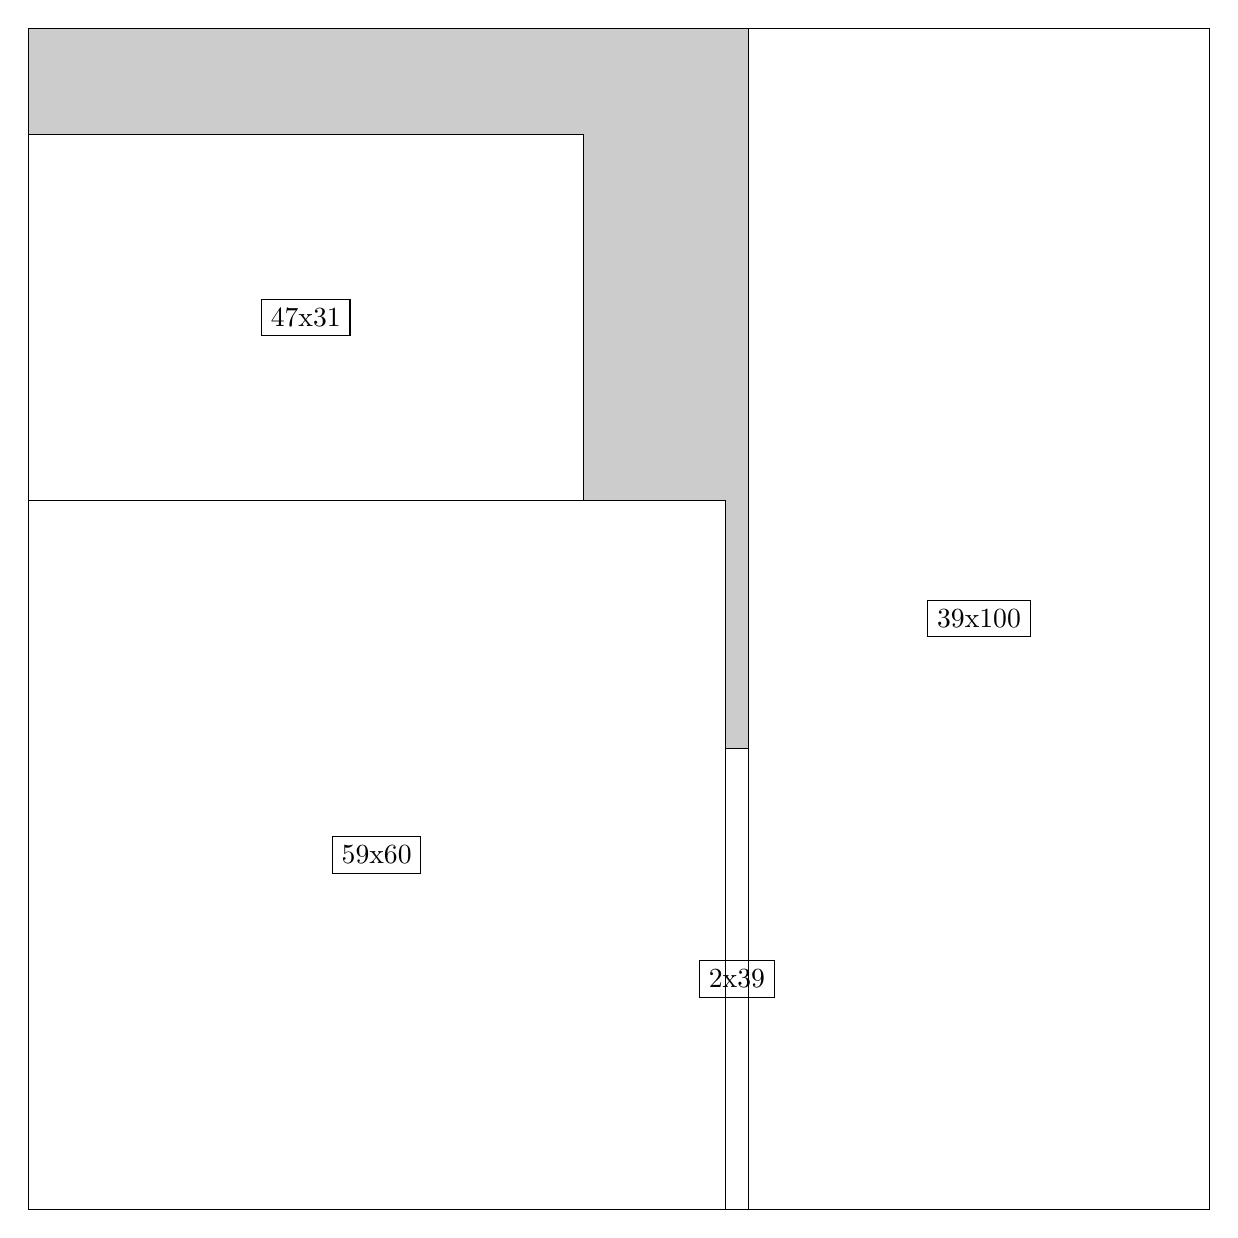
\begin{tikzpicture}[shorten >=1pt,scale=1.0,every node/.style={scale=1.0},->]
\tikzstyle{vertex}=[circle,fill=black!25,minimum size=14pt,inner sep=0pt]
\filldraw[fill=gray!40!white, draw=black] (0,0) rectangle (15.0,15.0);
\foreach \name/\x/\y/\w/\h in {59x60/0.0/0.0/8.85/9.0,47x31/0.0/9.0/7.05/4.6499999999999995,39x100/9.15/0.0/5.85/15.0,2x39/8.85/0.0/0.3/5.85}
\filldraw[fill=white!40!white, draw=black] (\x,\y) rectangle node[draw] (\name) {\name} ++(\w,\h);
\end{tikzpicture}


w =59 , h =60 , x =0 , y =0 , v =3540
\par
w =47 , h =31 , x =0 , y =60 , v =1457
\par
w =39 , h =100 , x =61 , y =0 , v =3900
\par
w =2 , h =39 , x =59 , y =0 , v =78
\par
\newpage


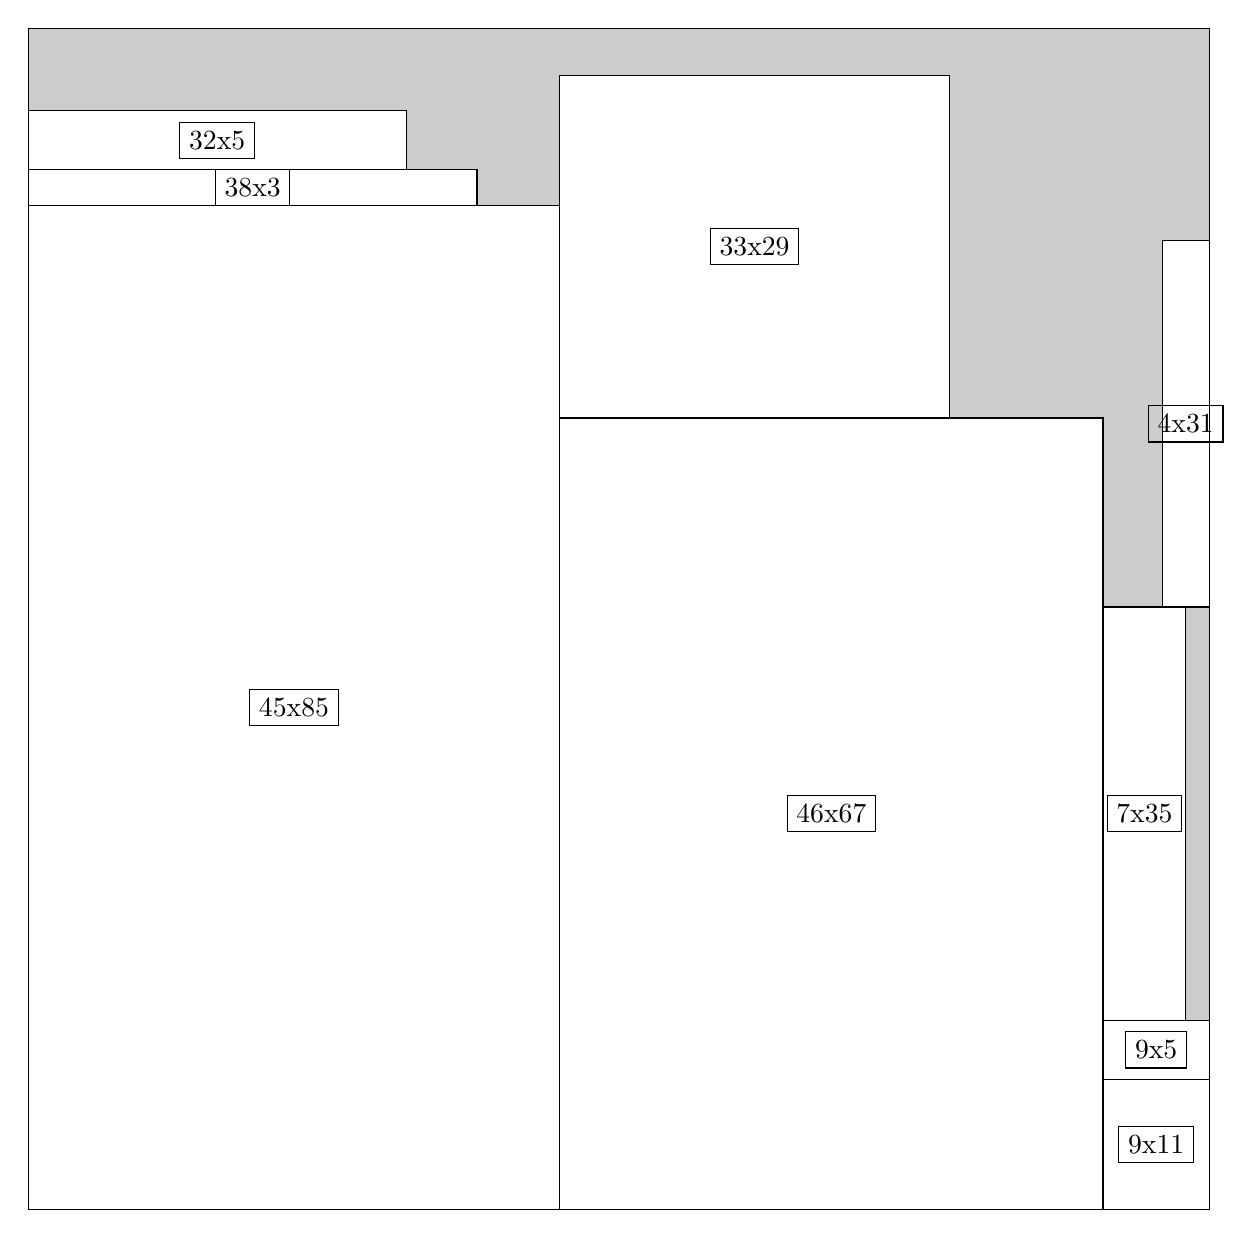
\begin{tikzpicture}[shorten >=1pt,scale=1.0,every node/.style={scale=1.0},->]
\tikzstyle{vertex}=[circle,fill=black!25,minimum size=14pt,inner sep=0pt]
\filldraw[fill=gray!40!white, draw=black] (0,0) rectangle (15.0,15.0);
\foreach \name/\x/\y/\w/\h in {45x85/0.0/0.0/6.75/12.75,46x67/6.75/0.0/6.8999999999999995/10.049999999999999,33x29/6.75/10.049999999999999/4.95/4.35,7x35/13.65/2.4/1.05/5.25,32x5/0.0/13.2/4.8/0.75,4x31/14.399999999999999/7.6499999999999995/0.6/4.6499999999999995,38x3/0.0/12.75/5.7/0.44999999999999996,9x11/13.65/0.0/1.3499999999999999/1.65,9x5/13.65/1.65/1.3499999999999999/0.75}
\filldraw[fill=white!40!white, draw=black] (\x,\y) rectangle node[draw] (\name) {\name} ++(\w,\h);
\end{tikzpicture}


w =45 , h =85 , x =0 , y =0 , v =3825
\par
w =46 , h =67 , x =45 , y =0 , v =3082
\par
w =33 , h =29 , x =45 , y =67 , v =957
\par
w =7 , h =35 , x =91 , y =16 , v =245
\par
w =32 , h =5 , x =0 , y =88 , v =160
\par
w =4 , h =31 , x =96 , y =51 , v =124
\par
w =38 , h =3 , x =0 , y =85 , v =114
\par
w =9 , h =11 , x =91 , y =0 , v =99
\par
w =9 , h =5 , x =91 , y =11 , v =45
\par
\newpage


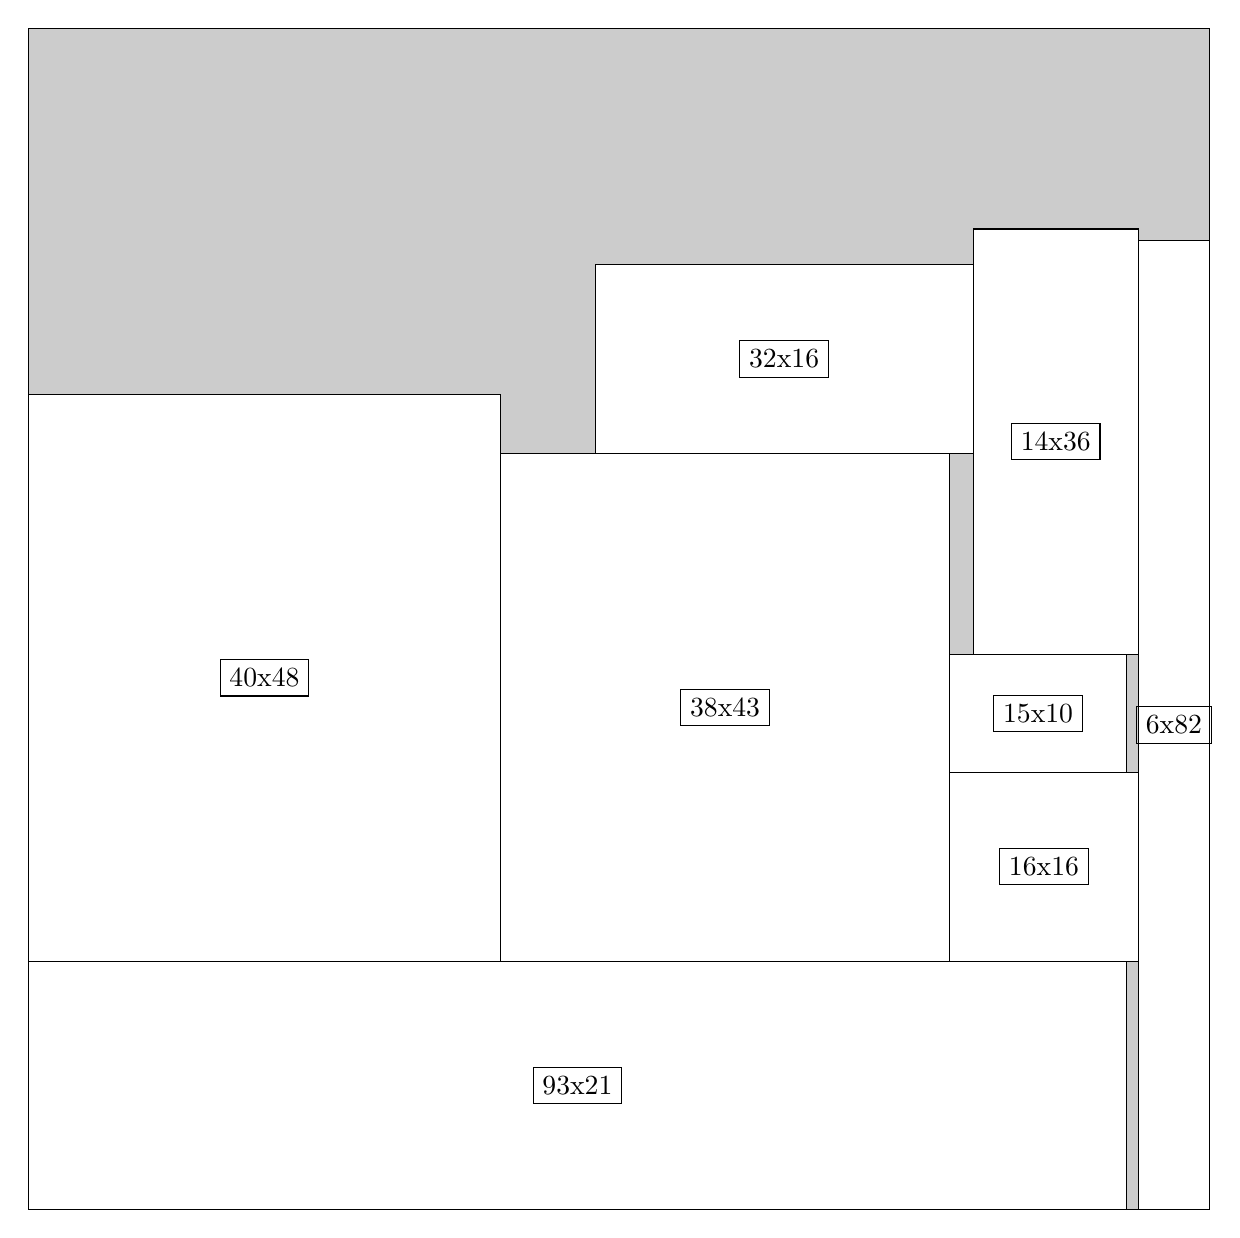
\begin{tikzpicture}[shorten >=1pt,scale=1.0,every node/.style={scale=1.0},->]
\tikzstyle{vertex}=[circle,fill=black!25,minimum size=14pt,inner sep=0pt]
\filldraw[fill=gray!40!white, draw=black] (0,0) rectangle (15.0,15.0);
\foreach \name/\x/\y/\w/\h in {93x21/0.0/0.0/13.95/3.15,40x48/0.0/3.15/6.0/7.199999999999999,38x43/6.0/3.15/5.7/6.45,32x16/7.199999999999999/9.6/4.8/2.4,14x36/12.0/7.05/2.1/5.3999999999999995,6x82/14.1/0.0/0.8999999999999999/12.299999999999999,16x16/11.7/3.15/2.4/2.4,15x10/11.7/5.55/2.25/1.5}
\filldraw[fill=white!40!white, draw=black] (\x,\y) rectangle node[draw] (\name) {\name} ++(\w,\h);
\end{tikzpicture}


w =93 , h =21 , x =0 , y =0 , v =1953
\par
w =40 , h =48 , x =0 , y =21 , v =1920
\par
w =38 , h =43 , x =40 , y =21 , v =1634
\par
w =32 , h =16 , x =48 , y =64 , v =512
\par
w =14 , h =36 , x =80 , y =47 , v =504
\par
w =6 , h =82 , x =94 , y =0 , v =492
\par
w =16 , h =16 , x =78 , y =21 , v =256
\par
w =15 , h =10 , x =78 , y =37 , v =150
\par
\newpage


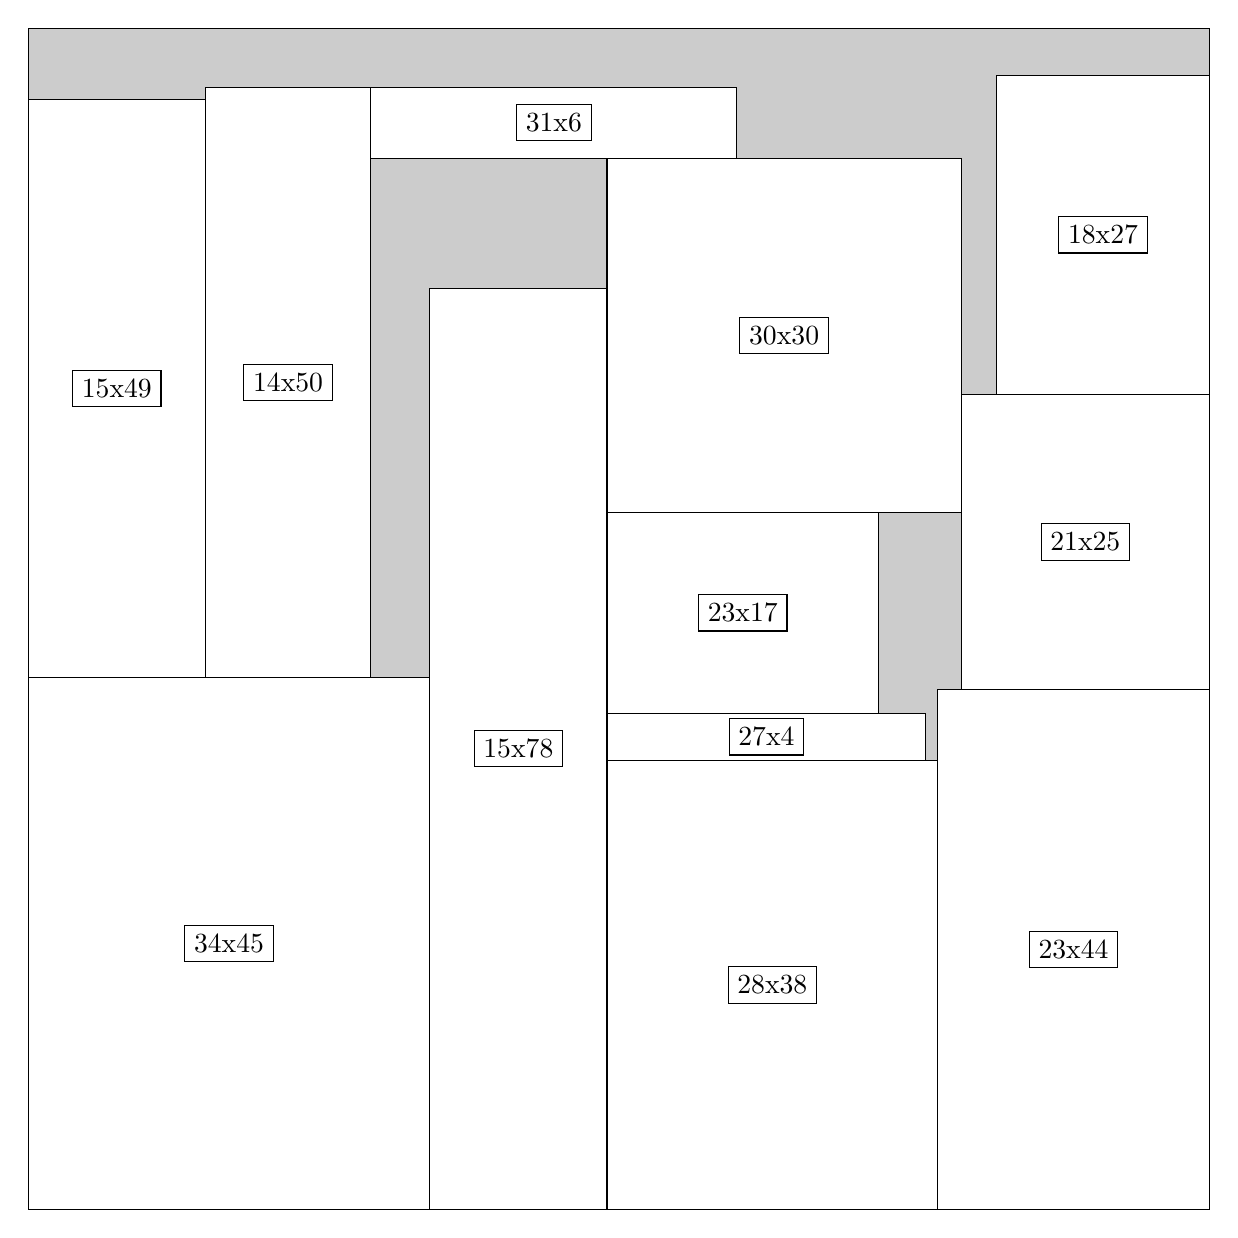
\begin{tikzpicture}[shorten >=1pt,scale=1.0,every node/.style={scale=1.0},->]
\tikzstyle{vertex}=[circle,fill=black!25,minimum size=14pt,inner sep=0pt]
\filldraw[fill=gray!40!white, draw=black] (0,0) rectangle (15.0,15.0);
\foreach \name/\x/\y/\w/\h in {34x45/0.0/0.0/5.1/6.75,15x78/5.1/0.0/2.25/11.7,28x38/7.35/0.0/4.2/5.7,23x44/11.549999999999999/0.0/3.4499999999999997/6.6,30x30/7.35/8.85/4.5/4.5,15x49/0.0/6.75/2.25/7.35,14x50/2.25/6.75/2.1/7.5,21x25/11.85/6.6/3.15/3.75,18x27/12.299999999999999/10.35/2.6999999999999997/4.05,23x17/7.35/6.3/3.4499999999999997/2.55,31x6/4.35/13.35/4.6499999999999995/0.8999999999999999,27x4/7.35/5.7/4.05/0.6}
\filldraw[fill=white!40!white, draw=black] (\x,\y) rectangle node[draw] (\name) {\name} ++(\w,\h);
\end{tikzpicture}


w =34 , h =45 , x =0 , y =0 , v =1530
\par
w =15 , h =78 , x =34 , y =0 , v =1170
\par
w =28 , h =38 , x =49 , y =0 , v =1064
\par
w =23 , h =44 , x =77 , y =0 , v =1012
\par
w =30 , h =30 , x =49 , y =59 , v =900
\par
w =15 , h =49 , x =0 , y =45 , v =735
\par
w =14 , h =50 , x =15 , y =45 , v =700
\par
w =21 , h =25 , x =79 , y =44 , v =525
\par
w =18 , h =27 , x =82 , y =69 , v =486
\par
w =23 , h =17 , x =49 , y =42 , v =391
\par
w =31 , h =6 , x =29 , y =89 , v =186
\par
w =27 , h =4 , x =49 , y =38 , v =108
\par
\newpage


\end{document}